\documentclass[sigconf,natbib=false,10pt]{acmart}

%%
%% \BibTeX command to typeset BibTeX logo in the docs
\AtBeginDocument{%
	\providecommand\BibTeX{{%
			Bib\TeX}}}

%% Rights management information.  This information is sent to you
%% when you complete the rights form.  These commands have SAMPLE
%% values in them; it is your responsibility as an author to replace
%% the commands and values with those provided to you when you
%% complete the rights form.
%\setcopyright{acmlicensed}
%\copyrightyear{2018}
%\acmYear{2018}
%\acmDOI{XXXXXXX.XXXXXXX}

%% Bibliography style
\RequirePackage[datamodel=acmdatamodel,style=acmnumeric]{biblatex}

%% Declare bibliography sources
\addbibresource{reference.bib}

%%
%% end of the preamble, start of the body of the document source.
\begin{document}
	
	%%
	%% The "title" command has an optional parameter,
	%% allowing the author to define a "short title" to be used in page headers.
	\title{Assistant Tools and Accessibility Features for Blind People Playing Visual-Centric Digital Games}
	
	\author{Marco Prescher}
	%\authornote{This is a author note!}
	\affiliation{%
		\institution{FHV University of Applied Sciences}
		\streetaddress{Hochschulstraße 1}
		\city{Dornbirn}
		\state{Vorarlberg}
		\country{Austria}}
		\postcode{6850}
	\email{marco.prescher@students.fhv.at}
	
	%%
	%% By default, the full list of authors will be used in the page
	%% headers. Often, this list is too long, and will overlap
	%% other information printed in the page headers. This command allows
	%% the author to define a more concise list
	%% of authors' names for this purpose.
	\renewcommand{\shortauthors}{Marco Prescher}
	
	%%
	%% The abstract is a short summary of the work to be presented in the
	%% article.
	%TODO
	\begin{abstract}
		Lorem ipsum dolor sit amet, consectetur adipiscing elit. Morbi
		malesuada, quam in pulvinar varius, metus nunc fermentum urna, id
		sollicitudin purus odio sit amet enim. Aliquam ullamcorper eu ipsum
		vel mollis. Curabitur quis dictum nisl. Phasellus vel semper risus, et
		lacinia dolor. Integer ultricies commodo sem nec semper.
	\end{abstract}
	
	\ccsdesc[500]{Applied computing~Computer games}
	\ccsdesc[500]{Human-centered computing~Accessibility}
	\ccsdesc[500]{Human computer interaction (HCI)}
	
	%%
	%% Keywords. The author(s) should pick words that accurately describe
	%% the work being presented. Separate the keywords with commas.
	\keywords{blind, accessibility, gaming, digital games, navigation, tools, AI}
	
	%\received{20 February 2007}
	%\received[revised]{12 March 2009}
	%\received[accepted]{5 June 2009}
	
	%%
	%% This command processes the author and affiliation and title
	%% information and builds the first part of the formatted document.
	\maketitle
	
	\section{Introduction}
	Today's accessible games for blind people are mainly games which are directly developed for them (\textcite{goncalves_my_2023}).
	While these games are enjoyable, mainstream games are a serious challenge for blind people because they consist of complex environments, mechanics and interactions with \emph{Non-Player Character} (NPC) players or even real players in \emph{Player versus player} (PvP) games.
	
	Implementing accessibility features is much needed in digital games to ensure that everyone, including people with disabilities can enjoy gaming.
	However, game developers in general face various problems in the process of developing games, some of them are:
	
	\begin{itemize}
		\setlength\itemsep{0.5em}
		\item Diverse Needs
		\item Technical Challenges
		\item Design Compromises
		\item Standardization
	\end{itemize}
	
	So, the main idea of this paper is to give a broad insight of different and innovative accessibility features and tools, including haptic feedback and its ways to improve game experience which is a major technical challenge.
	Additionally, this study explores design compromises and their associated problems as well as the need for standardization in the gaming industry developing games.
	This raises two relevant research questions (RQ):
	
	\begin{itemize}
		\setlength\itemsep{0.5em}
		\item RQ1: Which innovative accessibility features and tools can enhance the gaming experience for blind players?
		\item RQ2: In what ways can haptic feedback enhancements improve the game experience for blind players?
	\end{itemize}

	%TODO
	Contributions...

	\subsection{Motivation}
	One big step forward making mainstream games more accessible for blind people was the game \emph{The Last of Us Part II} (TLOU2) \cite{playstation_last_2020, playstation_last_2020-1}. 
	According to \textcite{leite_extended_2021} the game company \emph{Naughty Dog} implemented more than 60 accessibility features and is considered as the most accessible game ever produced.
	Additionally, \textcite{dale_last_2024} described that the game can be played all the way through with audio cues and navigation aids.
	It includes preset accessibility options for common disabilities like hearing or vision impairments. 
	It also introduces accessibility menus when the game is first started, making it easier for players with disabilities to adjust settings.
	To top that, \emph{Naughty Dog} released a remastered version of TLOU2 in 2024 with a reworked \emph{Cinematic Audio Descriptions} feature \cite{playstation_last_2024}.
	
	\section{The Problem}
	Blind players encounter many different barriers when playing visual-centric digital games which often rely greatly on graphical interfaces and visual cues. 
	To top that, the collection of those mainstream games have different perspectives such as top-down, first-person, and third-person views, where all three views give the player unique challenges in navigating game environment, understanding game objectives and interacting with in-game elements like players or objects.
	Building on that, the authors of \textcite{goncalves_my_2023} have categorized seven themes and identified unresolved barriers (see \autoref{fig:seven-themes}) which still represent a great challenge for both players and developers.
	%TODO rewrite
	
	\begin{figure*}[ht]
		\centering
		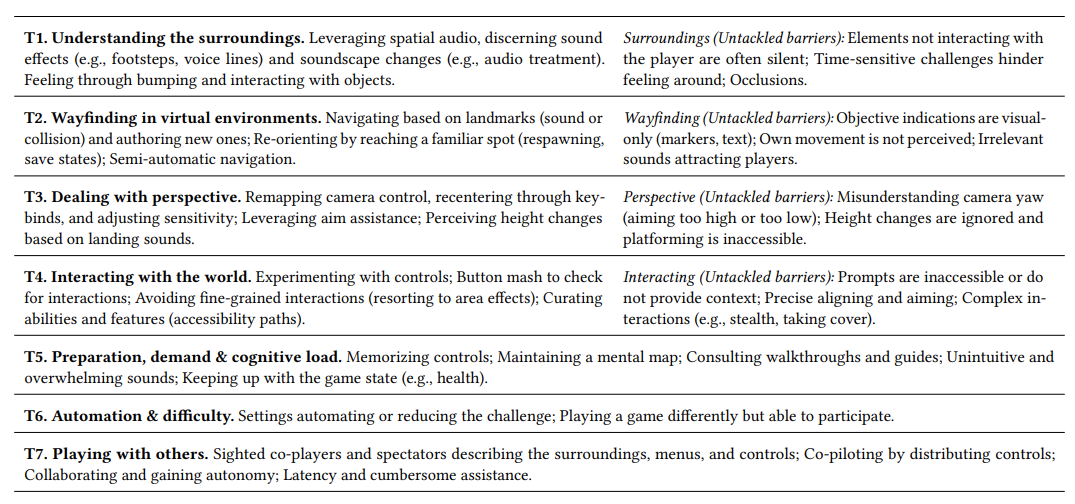
\includegraphics[scale=0.6,width=\textwidth]{assets/seven-themes.png}
		\caption{Seven themes and respective unresolved barriers (Source: \textcite{goncalves_my_2023})}
		\label{fig:seven-themes}
	\end{figure*}

	\autoref{fig:seven-themes} gives a great overview what accessibility features and assistant tools are still missing and in which direction the gaming industry should focus.
	
	\section{My Idea}
	The gaming industry came a long way from no accessibility features and assistant tools at all to implementing more than 60 accessibility features in one game \cite{playstation_last_2020}.
	According to research papers \cite{goncalves_my_2023, grammenos_designing_2009, grammenos_game_2008, araujo_mobile_2017} some of the most important accessibility features for blind people in visual-centric games include:
	
	\begin{itemize}
		\setlength\itemsep{0.5em}
		\item Audio Cues and Descriptions
		\item \emph{Text-to-Speech} (TTS) and Voiceover
		\item Navigation Aids and Wayfinding Tools
		\item Comprehensive Audio Design
		\item Customizable Controls and Inputs
		\item Tactile Feedback and Controller Design
	\end{itemize}
    
    Some of these have already been implemented to a certain extent in some games, but as \autoref{fig:seven-themes} notes, there are still problems.
    Especially when it comes to the environment, pathfinding, perspective and interacting with the world, blind players face major challenges, which according to \textcite{goncalves_my_2023} could mean they stop playing these games because they simply can not find the right way to play.
    
    To address the environment and pathfinding problems, one new technology was introduced in 2018 by \textcite{andrade_echo-house_2018} to use echolocation to explore a virtual environment which could drastically improve navigation in it.
    As for perspective (camera) and interacting with the world, hardware solutions like haptic feedback or AI assistant tools could be a solution when developed and integration further.
    Whereas the haptic feedback \cite{bello_haptics_2016} of for example PS5-Controllers \cite{akyaman_anticipated_2021, chen_gamepad_2024} could indicate when players aim too high or too low while an AI tool could provide the player with enhanced audio descriptions and how to interact with the world.
    
    In summary, it can be said that the game industry already takes into account the most important accessibility features, yet most modern visually-centric digital games are still a major challenge for blind players.
    In the following section we will delve deeper into some of the listed features above, their problems and possible solutions, as well as how to improve the overall experience of blind people.
	
	\section{Related Work}
	As digital games continuous to evolve making them more complex to play, accessibility becomes increasingly more important.
	This section provides a deeper insight in related works that contributed to the understanding of how important accessibility in visual-centric digital games is.
	
	\subsection{Themes of accessibility}
	The paper \textcite{goncalves_my_2023} explores the strategies blind players use to play visual-centric mainstream games.
	It analyzes over 70 hours of YouTube content from blind players to identify the strategies and methods they use to navigate and interact within games environments.
	
	The study highlights that blind players often rely on audio cues to understand and navigate game environments.
	They use repetitive actions like bumping into a wall to create a mental map of the environment.
	Players also try to create landmarks by interacting with the game world, for example, by leaving enemies behind to know in which area they are at the moment.
	This approach helps to navigate in game environments but also scare of new blind players due to frustration if the player become disorientated.
	
	The result of their findings are seven themes focusing on describing strategies blind players created and adopted: (See \autoref{fig:seven-themes})
	
	\begin{itemize}
		\setlength\itemsep{0.5em}
		\item Understanding the surroundings
		\item Wayfnding in virtual environments
		\item Dealing with perspective
		\item Interacting with the world
		\item Preparation, demand and cognitive load
		\item Automation and difficulty
		\item Playing with others
	\end{itemize}

	Additionally, \autoref{fig:seven-themes} shows us the existing barriers mainstream games have.
	
	The paper also acknowledges the efforts of some game developers to make new and existing games more accessible to blind players.
	This approach by developers is essential for reducing the accessibility gap in the upcoming years of game development.
	
	\subsection{Inaccessibility in Games}
	In 2008 \textcite{grammenos_game_2008} developed a game called \emph{Game Over!}, which is the first universally inaccessible game, created as an educational tool to teach game developers about accessibility guidelines.
	This approach aimed to raise awareness and motivate game developers to make their games accessible for everyone.
	
	The developed game \emph{Game Over!} has 21 levels implemented, each one violating a specific game accessibility guideline to frustrate but also educate by directly showing the developer what impact their design decisions have. 
	Some of the guidelines are:
	
	\begin{itemize}
		\setlength\itemsep{0.5em}
		\item Require complex key combinations
		\item Rapidly changing control schemes
		\item Presenting information in inaccessible formats
	\end{itemize}

 	Collected feedback from developers and players through surveys and public discussions indicate that the game raises awareness and educates about accessibility as intended.
 	It also suggested for the game to include direct access to additional information about each violated guideline, such as how specific accessibility can improve the game experience for disabled players.
 	
 	The feedback also highlighted to add more levels to cover a wider range of accessibility guidelines which would add the potential to adapt the concept and further improve it as well as to highlight the importance of game design in digital games.
	
	\subsection{Navigate a virtual environment using echolocation}
	In 2018 \textcite{andrade_echo-house_2018} investigates the use of echolocation in a game environment to help blind players to navigate in them.
	This approach aimed to investigate whether it is possible to create a \emph{virtual environment} (VE) where players can simulate echolocation to navigate and understand complex scenes within that VE.
	
	Therefore, they developed a VE with Unity 5.6 and the SteamAudio plug-in.
	This VE basically represents a three level house called \emph{Echo-House}, where users can navigate using sounds such as mouth-clicks, claps and footsteps, which generate echoes to receive information about the environment.
	Each level had a goal players needed to reach to get to the next level of the house (See \autoref{fig:echo-house-layout}).
	
	\begin{figure}[ht]
		\centering
		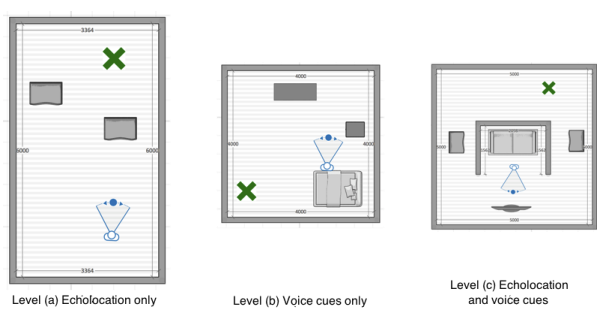
\includegraphics[scale=0.5]{assets/echo-house-layout.png}
		\caption{Layout of the three levels (Source: \textcite{andrade_echo-house_2018})}
		\label{fig:echo-house-layout}
	\end{figure}

	The evaluation consists of a 45-minute playing session and a interview.
	They found out that the echolocation provided the player with an improved sense of space within the VE.
	However, challenges in orientation and mobility were still present which indicates the need of further support.
	
	The paper highlighted the limitation of the study such as the small sample size and the need for further research to validate their findings.
	Nevertheless, this paper gives important insight of what can be achieved with echolocation to help blind players.
	
	
	\section{The Details}
	In this section, we delve into enhancing accessibility in digital games for blind players.
	Firstly, we aim to explore previously mentioned developing problems, from universally accessible game design affecting diverse needs followed by technical challenges.
	Secondly, we explore various types of feedback which are essential in enhancing of accessibility in digital games and focus on haptic feedback as well as further possibilities to use that to improve the experience in digital games for blind players.
	Lastly, we propose enhancements of already existing accessibility features and tools.
	
	\subsection{Universally Accessible Game Design}
	In recent years, the awareness of accessible game design has been growing tremendously.
	According to \emph{World Health Organization} \cite{world_health_organization_international_2004}, one out of ten persons has disabilities which often results in limitations in hearing, memory, vision or motor functions.
	
	Digital games are getting more demanding in terms of the limitations we described before and this is where \emph{Universally Accessible Game Design} (UAGD) comes into play.
	Through the implementation of UAGD, players with disabilities can benefit from features such as support for alternative input devices, including switches, eye-tracking systems, and mouth-operated controllers, which as a result can drastically enhance the game experience.
	One of the key aspects is the implementation of settings that allow players to customize the features they need to improve their game experience.
	
	We found a promising user-centered approach in the paper \textcite{grammenos_unified_2007} to apply UAGD in the development cycle of games.
	The basic steps are summarized in \autoref{fig:universal-game-design-approach}, whereas an elaboration of these is provided in \textcite{grammenos_unified_2007}.
	
	\begin{figure}[ht]
		\centering
		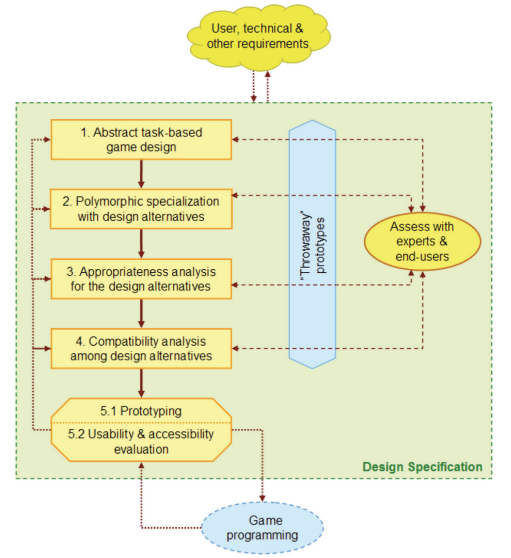
\includegraphics[scale=0.5]{assets/universal-game-design-approach.png}
		\caption{Applying UAGD (Source: \textcite{grammenos_unified_2007})}
		\label{fig:universal-game-design-approach}
	\end{figure}
	
	\subsection{Assistive haptic feedback}
	%TODO
	Short introduction into feedback variants and where it is used "visual perception (sight), haptics (tactile) and aural (hearing)". \cite{kuber_towards_2007}
	
	\subsection{Further possibilities to use haptic feedback}
	%TODO
	Combination with echolocation?
	
	\subsection{Ways to improve existing accessibility features and tools}
	%TODO
	AI-tools?
	
	\section{Conclusions and Further Work}
	%TODO
	A recap of the problem addressed and the proposed solution.
	The implications of your research for the gaming industry and the broader accessibility community.
	Any remaining challenges or unanswered questions that need to be addressed.
	Suggestions for future research directions or enhancements to your proposed idea.
	How your work contributes to advancing the state-of-the-art in accessibility technology for blind individuals playing digital games.
	
	
	%%
	%% Print the bibliography
	%%
	\printbibliography
	
\end{document}